\section{Implementation}
\label{sec:impl}
\subsection{Cross-Compilation}
Nearly all modern smartphones run arm processors.  On the other hand, nearly all modern desktops run x86 or x86\_64 processors. As a result of the architectural differences, binaries created in normal desktop PC environments will not work on smartphones. Additionally, the devices themselves are rather limited with respect to building code.  Relatively limited cpu, memory, disk, coupled with input and usability concerns make this an unattractive way to compile code.  A number of devices have lacking userspace environments that would make compiling code on them even more difficult.
Our solution is to use a cross-compileration environment to use a faster desktop to write our code targetting the various mobile platforms.
We build upon the scratchbox2 enviroment \cite{sb2}, in particular using the cross-compilation enviroment created by webos-internals \cite{webosinterals}.\\
Scratchbox2 is a cross-compilation engine that uses a combination of emulation and library interposition to make it easier to cross-compile code bases that don't otherwise provide a means to cross-compile.
The result is almost a virtualized environment that automatically invokes cross-compilation tools as required, abstracting away much of difficulies that cross-compilation can usually entail.
Important features in our environment include 1)a system of dependency resolution that allows us to conveniently build and package our applications more easily; 2)staging headers and device libraries such that we can use the same ones that are available on the target device; 3)static or dynamically linked executable compilation.
This allows us to conveniently build for multiple platforms from the comfort and reliabilty of our own systems.  Presently we use this to target the Palm Pre as well as android devices, in particular the Motorola G1.

\subsection{libc vs bionic}
Despite the fact the Pre and the Android are both running Linux OSes on an arm chip, the environments they provide for our project are enormously different.  The Pre is bundled with a large suite of common Unix applications and libraries, while the Android diverges, running minimalistic libraries and lacking many common libraries and applications.  Of these differences, the C compiler library is probably the most substantial. The Pre uses an unmodified version of glibc and the Android uses Bionic, a lightweight and small C compiler library.  Many Linux applications have glibc as a dependency, and as a result, builds for the Android must have statically link libraries.  Between this and the lack of useful applications (gdb and other debugging tools) development on the Android has provent much more difficult.  

\subsection{X-Server}

We made a number of important design decisions, many of which were in response to unexpected implementation difficulties.  The result of our X server (including a fixed Xsdl implementation) work is available on the website.
\subsubsection{DDX}
The X-Server architecture contains multiple Device Dependent X (DDX) implementations.  The most used one is 'xfree86', but there are others including 'kdrive' \cite{x_glossary}.  We chose to use kdrive because of the Xsdl component it contains, which allows one to run X using SDL as a backend.  Unfortunately Xsdl is so out of date that it was recently removed from the X project altogether due to being broken and unmaintained.
From X version control: ``if anyone uses this in production, a big scary monster will eat them'' \cite{x_quote}.  The result of this was much work spending fixing Xsdl and bringing it up to date to work with the rest of X.  Fixes including interactions with the X server, as well as fixing the rendering code and the input handling.
\subsubsection{SDL and GLES}
As described above, the code we started with used Simple DirectMedia Layer (SDL) \cite{sdl} for input and rendering.  Once we had achieved this functionaliy, we noticed the display lagged when doing even basic things like moving the cursor.  Previous experience working with SDL on this device suggested that using GLESv2 \cite{gles} and custom shaders would improve a task even as simple as blitting, so we ported the rendering bits to use GLESv2.

\subsubsection{Devices that don't support SDL}
Although the Pre has support for SDL, many devices don't, and that's something we've taken into consideration.  The kdrive structure can be made rather portable: at it's heart it just needs something that can render a pixelbufer, and feed it input (either event driven or by polling).  This means that we could potentially support Android devices through Java Native Interface (JNI) \cite{jni} passing the buffer to a java app to blit and the java app blitting to the screen, as well as gathering input and feeding it to the X server.
\subsubsection{Keyboard}
Keyboard support is very important when using applications.  However it was a stumbling block for us two main reasons: 1)mapping SDL to something the X server can use 2)adding support for keys and features that are not on the original device.\\
It is common for keyboards, particularly on phones, to have each key have multiple uses when pressed with a special modifier.  As an example, on the Pre, 'orange' plus 'q' is the '/' key.  This presented a problem because this means capturing the modifier requires creating a state machine to process the input as opposed to a simple lookup table.  We ended up using xkb to do this, and the results are in the xkeyboard-config git repository. \\
The second issue is that many keys that are required for doing something as simple as using 'xterm' simply don't exist on most phones.  Examples of such characters include the pipe '|' character, '>', '<', arrow keys, and more.  We currently support many such keys on the pre through more customizations to the xkb layout and hope to support other devices as we add support for them as well.
\subsubsection{Future: Integrating even more}
A primary goal of our project is to cleanly integrate into the host X server.  While our current implementation is a great step and does integrate as a window in the existing windowing system for the device, there is an issue.  Presently the X server will render everything into one window (see Figure \ref{fig:x_screenie}), which requires a window manager to manage the windows.  This is bad both because it is hard to use but also because it is a hard break from the goal of integrating with the parent window manager--now the user has to think about it as two separate systems.\\

One solution to this is to take advantage of the work done on rootless X \cite{rootless}.  ``The generic rootless layer allows an X server to be implemented on top of another window server in a cooperative manner. This allows the X11 windows and native windows of the underlying window server to coexist on the same screen. The layer is called ``rootless'' because the root window of the X server is generally not drawn. Instead, each top-level child of the root window is represented as a separate on-screen window by the underlying window server'' \cite{rootless}.\\

Another idea is to take advantage of standard X notification events \cite{notifications} and hook into mobile device notification systems, which both WebOS and Android support. 

\begin{figure}[tbh]
\centering
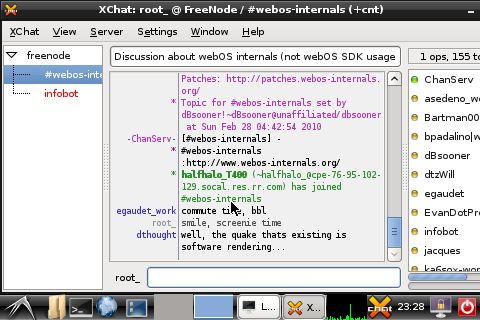
\includegraphics[width=1.0\columnwidth]{xchat1}
\caption{X server running icem and xchat}
\label{fig:x_screenie}
\end{figure}
